\section{Hardware Specifications}

All experiments were conducted on a high-performance
PC with the following specifications: 

\begin{itemize}
    \item CPU: Intel Core i7-9800X CPU @ 3.80GHz,
    3792 Mhz, 8 core, 16 threads
    \item GPU: 2 NVIDIA RTX 2080 Ti GPU with 12GB
    VRAM each
    \item RAM: 64 GB DDR4
    \item Storage: 1 TB Seagate BarraCuda HDD
\end{itemize}

\section{Software Environment}

The experiments were implemented using the following software stack:

\begin{itemize}
    \item Operating System: Windows 11 Pro
    \item Python: 3.10.14
    \item PyTorch: 2.3.0
    \item CUDA: 12.0
    \item TorchRL: 0.4.0
    \item MuJoCo: 3.14
\end{itemize}

\section{Network Architectures Details}

\subsection{WRe-CTDG Network Structure}

The WRe-CTDG framework consists of three main components:
Encoder $E_u$, Generator $G_s$, and Critic $C$.
Here are the details of each network:\\
\textbf{Encoder $\mathbf{E_u}$:}
\begin{itemize}
    \item Input layer: 2 $\times$ numerical state dimensions
    + 2 $\times$ latent state dimensions + action dimension
    \item Hidden layers: 4 fully connected layers with 256, 512, 512, and 256 units respectively
    \item Output layer: noise dimension + 1 (for reward prediction)
    \item Activation function: ReLU for hidden layers,
    Tanh/Sigmoid/Identity for reward output, Linear for noise output
\end{itemize}
\textbf{Generator $\mathbf{G_s}$:}
\begin{itemize}
    \item Input layer: numerical state dimension
    + latent state dimension + action dimension +
    noise dimension
    \item Hidden layers: 4 fully connected layers
    with 256, 512, 256, and 128 units respectively
    \item Output layer: numerical state dimension
    + latent state dimension
    \item Activation function: ReLU for hidden layers,
    Linear for output layer
\end{itemize}
\textbf{Critic $\mathbf{C}$:}
\begin{itemize}
    \item Input layer: 2 $\times$ numerical state dimensions
    + 2 $\times$ latent state dimensions + action dimension
    + noise dimension
    \item Hidden layers: 4 fully connected layers with 256,
    512, 256, and 128 units respectively
    \item Output layer: 1
    \item Activation function: ReLU
    for hidden layers, Linear for output layer
\end{itemize}
For environments with image inputs, we additionally used a
Convolutional AutoEncoder architecture to
encode and decode the state representations:\\
\textbf{Convolutional Encoder:}
\begin{itemize}
    \item 5 downsampling blocks
    \item Each block contains 2-3 convolutional layers
    with BatchNorm and ReLU activation
    \item Number of filters increases progressively:
    $$ in\_channels \rightarrow base \rightarrow 2
    \times base \rightarrow 4\times base \rightarrow
    8\times base \rightarrow 16\times base $$
    with $base = 8$.
    \item MaxPool2D with kernel size $2\times 2$ and stride
    2 for downsampling between blocks
    \item Final $1\times 1$ convolutional layer to
    reduce channel dimension to $bn = 1$ (bottleneck)
\end{itemize}
\textbf{Convolutional Decoder:}
\begin{itemize}
    \item Initial $1\times 1$ convolutional layer 
    to expand channel dimension from $bn$ to $16 \times base$
    \item 5 upsampling blocks
    \item Each block contains 2-3 convolutional
    layers with BatchNorm and ReLU activation
    \item Number of filters decreases progressively:
    $$ 16\times base \rightarrow 8
    \times base \rightarrow 4\times base \rightarrow
    2\times base \rightarrow base \rightarrow in\_channels$$
    with $base = 8$.
    \item Upsampling using transposed convolution
     with kernel size $2\times 2$ and stride 2
    \item Final layer uses Tanh activation
\end{itemize}
The encoder and decoder are symmetric, with the number of filters changing at each level.

\subsection{S-CTDG Network Structure}

The S-CTDG framework for \textbf{images} employs a network architecture
consisting of two components: a convolutional U-Net for counterfactual
image generation
and a separate convolutional network with a fully connected head for
reward prediction.\\
\textbf{U-Net}:
\begin{itemize}
    \item 5 downsampling blocks and 5 upsampling blocks
    \item Each block contains 2-3 convolutional layers
    with BatchNorm and ReLU activation
    \item Number of filters increases
    progressively in downsampling:
    $$ in\_channels \times (1 + stack\_length) + 2 \times (action\_channels)
    \rightarrow $$$$\rightarrow base \rightarrow 2
    \times base \rightarrow 4\times base \rightarrow
    8\times base \rightarrow 16\times base $$
    where the first term is the stack of current and previous images
    concatenated along the channel dimension with the next state image
    and the action and counterfactual action images.
    The number of filters then decreases in upsampling:
    $$ 16\times base \times 2 \rightarrow 8 \times base \times 2 \rightarrow
    4\times base \times 2\rightarrow$$ $$ \rightarrow 2\times base \times 2
    \rightarrow base \times 2 \rightarrow in\_channels$$
    with $base = 64$, in upsampling the filters are doubled
    since we concatenate the corresponding downsampling block.
    \item Convolution with kernel size $3\times 3$, stride 1,
    and padding 1
    \item MaxPool2D with kernel size $2\times 2$ and stride
    2 for downsampling between blocks
    \item Final layer uses a Softsign activation function
\end{itemize}
\textbf{Reward Prediction Network}:
\begin{itemize}
    \item 5 downsampling blocks
    \item Each block contains 2-3 convolutional layers
    with BatchNorm and ReLU activation
    \item Number of filters increases
    progressively in downsampling:
    $$ in\_channels \times (1 + stack\_length) + action\_channels
    \rightarrow base \rightarrow$$$$\rightarrow 2
    \times base \rightarrow 4\times base \rightarrow
    8\times base \rightarrow 16\times base $$
    where the first term is the stack of current and previous images
    concatenated along the channel dimension with the
    estimated counterfactual next state image
    and the counterfactual action image.
    As before, $base = 64$.
    \item Convolution with kernel size $3\times 3$, stride 1,
    and padding 1
    \item MaxPool2D with kernel size $2\times 2$ and stride
    2 for downsampling between blocks
    \item Final layer uses an Identity activation function
\end{itemize}

The S-CTDG framework for \textbf{numerical} data
employs a network architecture consisting of a single
fully connected network branched into two heads:
one for counterfactual data generation
and one for reward prediction.
The network architecture is as follows:
\begin{itemize}
    \item Input layer: 2 $\times$ numerical state dimensions
    $ + $ $2 \times $ action dimension
    \item Hidden layers: 7 fully connected layers with
    512, 512, 512 and 256 units respectively
    \item Output layer for counterfactual data generation:
    numerical state dimension, Linear activation function
    \item Output layer for reward prediction: 1,
    Identity activation function
\end{itemize}

\subsection{Reinforcement Learning Algorithms (D3QN and TD3)}

For the reinforcement learning algorithms, we used the following architectures:\\
For discrete action spaces we used \textbf{D3QN:}
\begin{itemize}
    \item Input layer: state dimension
    \item Hidden layers: 4 fully connected layers with 32, 64, 128 and 128
    units respectively
    \item Output layer: action dimension
\end{itemize}
It is a \textbf{Dueling CNN DQNetwork} as presented in \cite{d3qn}.\\
Then, for continuous action spaces we used \textbf{TD3:}\\
Actor:
\begin{itemize}
    \item Input layer: state dimension
    \item Hidden layers: 3 fully connected layers with 32, 64, 128 and 128
    units respectively
    \item Output layer: action dimension
    \item Activation function: ReLU for hidden layers, Tanh for output layer
\end{itemize}
Critic:
\begin{itemize}
    \item Input layer: state dimension + action dimension
    \item Hidden layers: 3 fully connected layers with 32, 64, 128 and 128
    units respectively
    \item Output layer: 1
    \item Activation function: ReLU for hidden layers, Linear for output layer
\end{itemize}
The actor and critic networks are modelled after
the architectures presented in \cite{lillicrap2019}. 

\section{Training Process Details}

\subsection{Dataset Generation}

For each environment, we generated a dataset of transitions using a random policy.
This dataset served as the basis for our counterfactual
data generation and reinforcement learning experiments.

The number of transitions in the dataset was different for each environment:
\begin{itemize}
    \item Acrobot: 20'000 transitions, observation stack length: 2
    \item Half Cheetah: 50'000 transitions, observation stack length: 4
    \item Ant: 50'000 transitions, observation stack length: 4
    \item Diabetes: 100 transitions, observation stack length: 1
\end{itemize} 

\subsection{Counterfactual Data Generation}

We used both WRe-CTDG and S-CTDG frameworks to generate counterfactual data.
The augmentation factor $\alpha$ was set to 4, effectively quadrupling
the size of the original datasets.
Only a subset of the original dataset
was used for generating counterfactual data.

Training parameters:
\begin{itemize}
    \item Batch size: 32
    \item Optimizer: Adam (learning rate: $1\times 10^{-4}$, $\beta_1$: 0.5, $\beta_2$: 0.9)
    \item Number of iterations: 10'000 for WRe-CTDG, 100'000 for S-CTDG\\
    (both $\approx 12$h of training)
    \item Frame size for image-based environments: $128\times 128$
\end{itemize}
Size of the augmented datasets:
\begin{itemize}
    \item Acrobot: 10'000 $\times \, \alpha =$ 40'000 transitions 
    \item Half Cheetah: 10'000 $\times \, \alpha =$ 40'000 transitions
    \item Ant: 10'000 $\times \, \alpha =$ 40'000 transitions
    \item Diabetes: 20 $\times \, \alpha =$ 80 transitions
\end{itemize}


\subsection{Reinforcement Learning Training}

We trained D3QN and TD3 algorithms on both the original and augmented datasets.
The training process involved:

\begin{itemize}
    \item Number of training steps: 1'000 for Acrobot, 3'000 for Half Cheetah, 6'000 for Ant
    \item Batch size: 256
    \item Discount factor ($\gamma$): 0.99
    \item Optimizer: Adam (learning rate: $1\times 10^{-4}$, $\beta_1$: 0.0, $\beta_2$: 0.9)
    \item Exploration strategy: $\epsilon$-greedy with decay factor $\tau = 0.005$
\end{itemize}

\section{Results}

\subsection{Reconstruction Loss During Generation}

We measured the Mean Absolute Error (MAE) on a validation set
between the generated counterfactual states and the ground truth
states after the training of WRe-CTDG (comparison between encoded values)
and S-CTDG (comparison between images) frameworks
as shown in Table \ref{tab:mae}.

\begin{table}[h]
\centering
\begin{tabular}{@{}lcc@{}}
    \toprule
    \textbf{Environment} & \textbf{WRe-CTDG MAE} & \textbf{S-CTDG MAE} \\ \midrule
    Acrobot              & 0.25189               & 0.00147             \\
    Half Cheetah         & 0.22064               & 0.03946             \\
    Ant                  & 0.27296               & 0.09391             \\
    Diabetes             & 0.                    & 0.                  \\ \bottomrule
    \end{tabular}
\caption{WRe-CTDG and S-CTDG Reconstruction Loss}
\label{tab:mae}
\end{table}

\subsection{Reinforcement Learning Performance}

We evaluated the performance of D3QN and TD3 algorithms on both the
original and augmented datasets. The results are presented
in \ref{tab:rl_reward} for reward values and \ref{tab:rl_loss}
for loss values: the reward value shown is the best reward
over all the evaluation episodes and 
the loss value is the loss at the time of the best reward.

\begin{table}[h]
    \centering
    \begin{tabular}{@{}llccc@{}}
        \toprule
        \textbf{Environment} & \textbf{Algorithm} & \textbf{No Aug.} & \textbf{S-CTDG Aug.} & \textbf{wRE-CTDG Aug.} \\ \midrule
        Acrobot              & D3QN               & -57.47           & -55.90                 & -53.35               \\
        Half Cheetah         & TD3                & 8.19             & 208.25                 & 311.25               \\
        Ant                  & TD3                & 67.33            & 180.78                 & 112.65               \\
        Diabetes             & D3QN               & -0.              & -0.                    & -0.                  \\ \bottomrule
    \end{tabular}
    \caption{Reinforcement Learning Best Reward Value}
    \label{tab:rl_reward}
\end{table}

\begin{table}[h]
    \centering
    \begin{tabular}{@{}llccc@{}}
        \toprule
        \textbf{Environment} & \textbf{Algorithm} & \textbf{No Aug.} & \textbf{S-CTDG Aug.} & \textbf{wRE-CTDG Aug.} \\ \midrule
        Acrobot              & D3QN               & 0.01157          & 0.00371                & 0.00368              \\
        Half Cheetah         & TD3                & 1.35503          & 2.81980                & 0.48767              \\
        Ant                  & TD3                & -0.94156         & -1.34450               & -14.13370            \\
        Diabetes             & D3QN               & -0.              & -0.                    & -0.                  \\ \bottomrule
    \end{tabular}
    \caption{Reinforcement Learning Loss Value during the Best Reward}
    \label{tab:rl_loss}
\end{table}

In Figure \ref{fig:rew_acrobot} we show the reward trends for the
Acrobot environment using D3QN, while in Figure \ref{fig:loss_acrobot}
we show the loss trends for the same environment.
In the case of Half Cheetah, we show the reward trends in
Figure \ref{fig:rew_cheetah} and the loss trends in
Figure \ref{fig:loss_cheetah}.
The trends of reward and loss values for the Ant environment
are shown in Figures \ref{fig:rew_ant} and \ref{fig:loss_ant} respectively.
At last, the trends for the Diabetes environment are shown in
Figures \ref{fig:rew_diabetes} and \ref{fig:loss_diabetes}.

\begin{figure}[h]
    \centering
    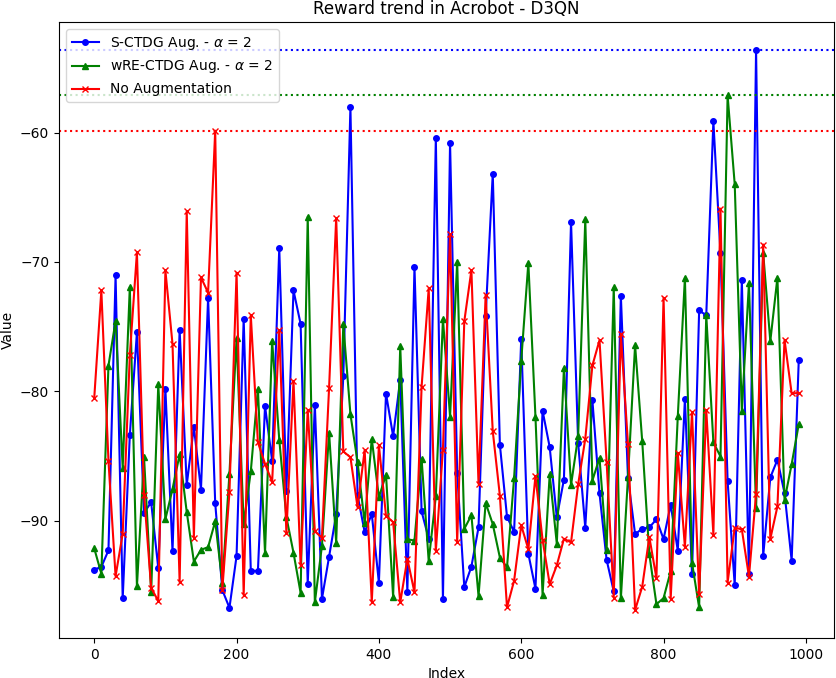
\includegraphics[width=.8\textwidth]{figures/ch5/rew_acrobot.png}
    \caption{Acrobot Reward Trends}
    \label{fig:rew_acrobot}
\end{figure}

\begin{figure}[h]
    \centering
    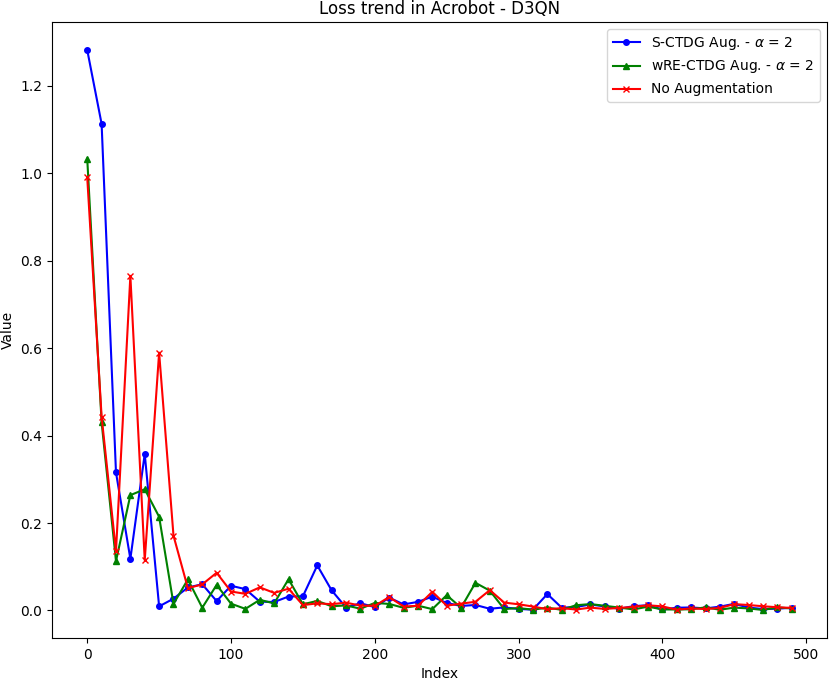
\includegraphics[width=.8\textwidth]{figures/ch5/loss_acrobot.png}
    \caption{Acrobot Loss Trends}
    \label{fig:loss_acrobot}
\end{figure}

\begin{figure}[h]
    \centering
    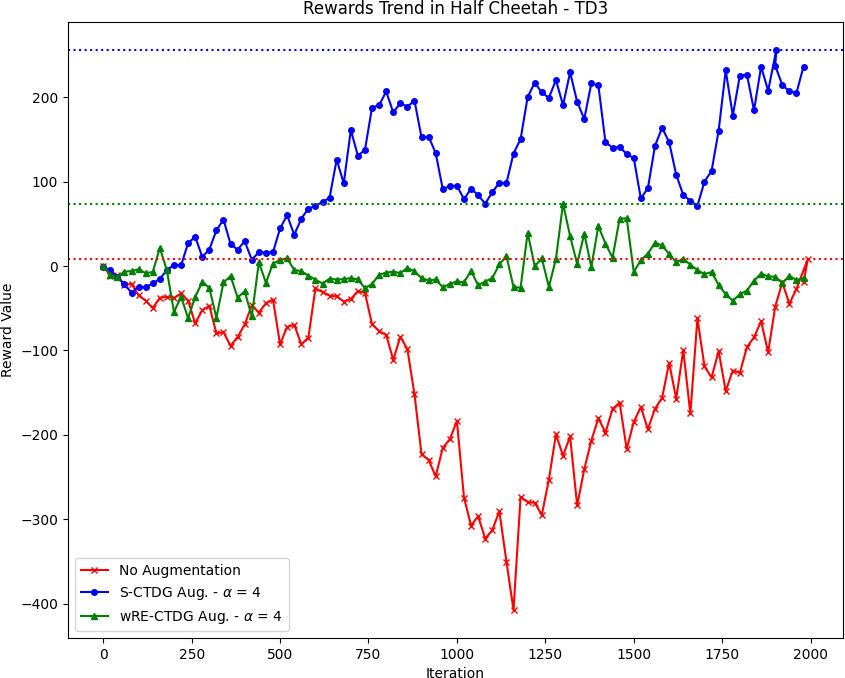
\includegraphics[width=.8\textwidth]{figures/ch5/rew_halfcheetah.png}
    \caption{Half Cheetah Reward Trends}
    \label{fig:rew_cheetah}
\end{figure}

\begin{figure}[h]
    \centering
    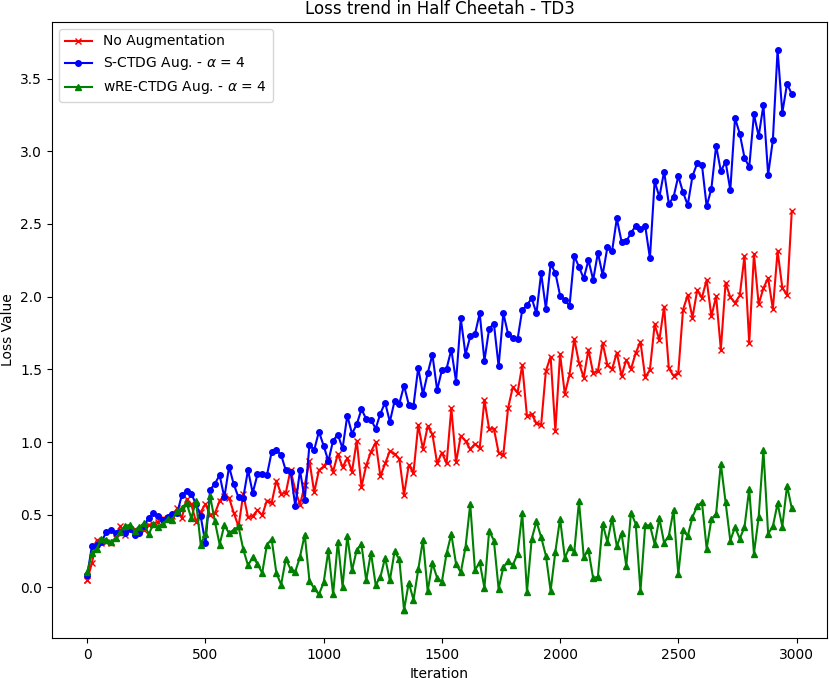
\includegraphics[width=.8\textwidth]{figures/ch5/loss_halfcheetah.png}
    \caption{Half Cheetah Loss Trends}
    \label{fig:loss_cheetah}
\end{figure}

\begin{figure}[h]
    \centering
    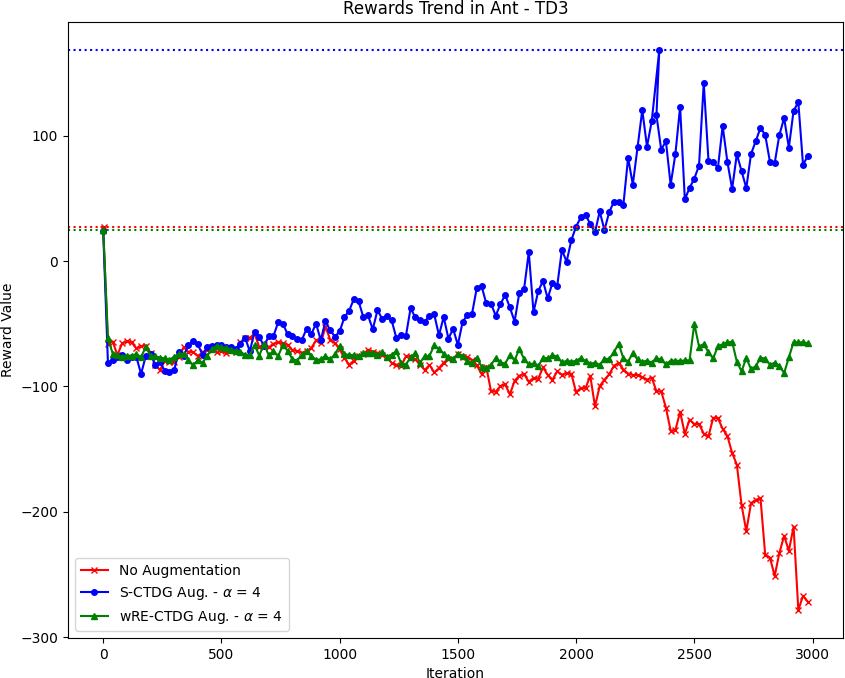
\includegraphics[width=.8\textwidth]{figures/ch5/rew_ant.png}
    \caption{Ant Reward Trends}
    \label{fig:rew_ant}
\end{figure}

\begin{figure}[h]
    \centering
    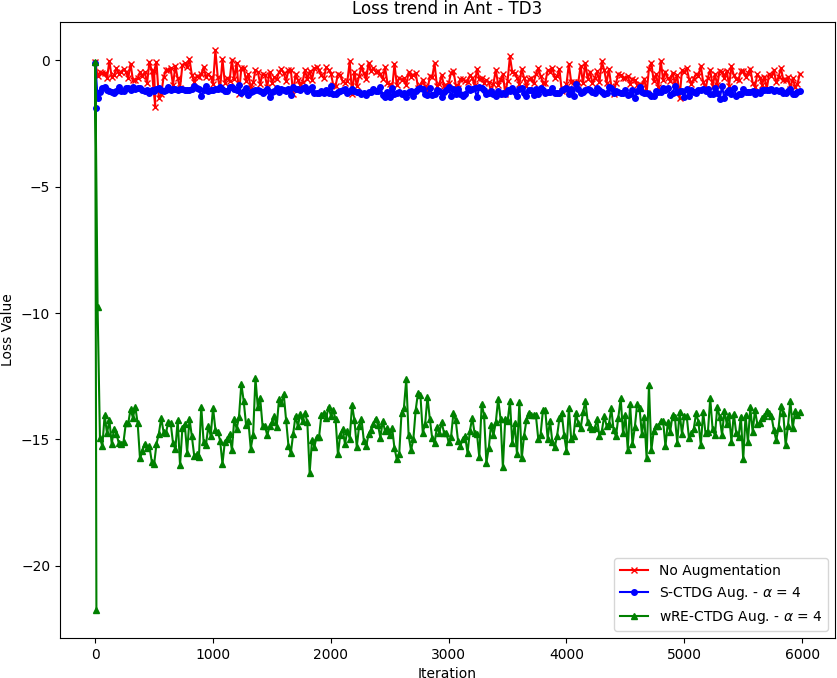
\includegraphics[width=.8\textwidth]{figures/ch5/loss_ant.png}
    \caption{Ant Loss Trends}
    \label{fig:loss_ant}
\end{figure}

